\chapter{Estado del Arte}
\label{cap:estadoDeLaCuestion}

Los humanos siempre  hemos tenido la necesidad inherente de comunicarnos y quien no es capaz de hacerlo, generalmente acaba excluido.

A día de hoy este problema sigue afectando a parte de la población como es el caso de las personas con trastorno del espectro autista (TEA).

Sin entrar en gran detalle, podemos encontrar que la gente con TEA tienen dificultades en la comunicación verbal pues a menudo la comunicación no es recíproca o no se realiza en el contexto social adecuado. Respecto a la comunicación no verbal, también sufren dificultades al entender el significado de gestos faciales o expresión corporal de otras personas. Todo esto causa a menudo malentendidos, pues generalmente no se comprende el contexto y dificulta la comunicación. 

Para facilitar la comunicación se utilizan otros medios alternativos, los SAAC.

\section{Sistemas Aumentativos y Alternativos de Comunicación}
Los Sistemas Aumentativos y Alternativos de Comunicación(SAAC) son las distintas formas de expresión sin tener en cuenta el lenguaje hablado que tiene como finalidad aumentar y/o compensar los problemas de comunicación de personas con discapacidad como por ejemplo trastornos del espectro autista, discapacidad intelectual, deficiencia auditiva, parálisis cerebral entre otros.

En ocasiones puede hacer falta el uso de recursos para poder comunicarse, es por ello que podemos distinguir dos tipos de SAACs, los sistemas sin ayuda y los sistemas con ayuda.
\newpage
\begin{itemize}
	\item Sistemas sin ayuda: no utilizan ningún recurso externo para establecer una comunicación, únicamente usan su propio cuerpo. En los sistemas sin ayuda podemos observar dos tipos de grupos, los métodos gestuales (lengua de signos) y los métodos oralistas (lectura labiofacial) . 
	\item Sistemas con ayuda: utilizan recursos externos para establecer una comunicación. Los más utilizados suelen ser pictogramas, imágenes o símbolos.
\end{itemize}

Las SAACs utiliza múltiples recursos para poder comunicarse con personas con discapacidades cognitivas y entre todos ellos destacan los sistemas pictográficos. Se trata de uno de los sistemas más utilizados y esto es debido a su fácil comprensión ya que representan gráficamente lo que se desea transmitir como palabras o conceptos. 

\section{Pictogramas}
Los pictogramas son imágenes o símbolos de rápida comprensión que expresan acciones, objetos, emociones etc. Un conjunto de pictogramas en orden, puede generar una oración. Todos ellos deben cumplir las siguientes características:
\begin{enumerate}
	\item Referencialidad: Busca la relación del pictograma con el referente.
	\item Ítems gráficos: imágenes que representen de manera sencilla aquello que se toma como modelo.
	\item Comprensión: debe ser fácilmente entendible independientemente de la formación, idioma o discapacidad.
	\item Legibilidad: Mantiene una coherencia visual entre pictogramas.
	\item Sencillez: Muestra únicamente los elementos relevantes sin elementos distractores o adornos insignificantes.
\end{enumerate}

\subsection{Sistemas pictográficos}
Existen numerosos sistemas pictográficos a continuación hablaremos de los más importante:

\subsubsection{Sistema pictográfico de comunicación}

Creado en 1981 por Roxana Mayer Johnson con la intención de facilitar la comunicación a quienes tienen un nivel de lenguaje expresivo simple o vocabulario limitado. Gracias a la diferenciación por colores, facilita la comprensión de la estructura sintáctica. Está organizado por seis colores según su función gramatical. Actualmente cuenta con más de 3000 iconos.

\begin{itemize}
	\item Personas (Amarillo): Representa a familiares y pronombres. Ejemplo: Mamá, familia,  yo, ellos.
	\item Verbos (Verde): Representan acciones. Ejemplo: Abrir, agarrar, comer, ir.
	\item Descriptivos (Azul): Descriptivos o adjetivos o adverbios
	\item Nombre (Naranja): Representan objetos u otros elementos que no aparecen en otra categoría. Ejemplo: Gato, Almohada o Casa.
	\item Miscelánea (Blanco): Representa números, letras y colores
	\item Social (Rosa): Vocabulario relacionado con relaciones sociales. Ejemplo: Buenos días, si, gracias, no lo sé.
	
\end{itemize}


% TODO: \usepackage{graphicx} required
\begin{figure}[h!]
	\centering
	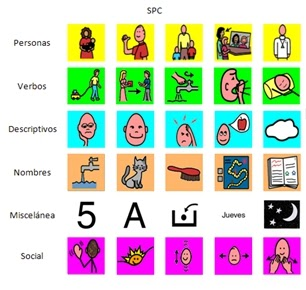
\includegraphics[width=0.7\linewidth]{Imagenes/Bitmap/SPCcolores}
	\caption{Ejemplo de categorías en Sistema Pictográfico de Comunicación}
	\label{fig:spccolores}
\end{figure}



